\begin{flushright} {\tiny {\color{gray} (tikz\_sv.tex)}} \end{flushright}
%~~~~~~~~~~~~~~~~~~~~~~~~~~~~~~~~~~~~~~~~~~~~~~~~~~~~~~~~~~~~~~~~~~~~~~~~~~~~~~~~~~~~~~~~~~~~~~~~~~


\begin{center} 
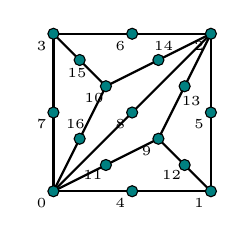
\begin{tikzpicture} 

%\draw[fill=gray!23,gray!23](0,0) rectangle (2.5,2.5);
%\draw[step=0.5cm,gray,very thin] (0,0) grid (2.5,2.5); %background grid

%ielx=1,iely=1,low
\draw[thick] (0,0)--(1.33333,0.66667);
\draw[thick] (2,0)--(1.33333,0.66667);
\draw[thick] (2,2)--(1.33333,0.66667);
%ielx=1,iely=1,high
\draw[thick] (0,0)--(0.666667,1.3333);
\draw[thick] (0,2)--(0.666667,1.3333);
\draw[thick] (2,2)--(0.666667,1.3333);

\draw[thick] (0,0) -- (2,0) -- (2,2) -- (0,2) -- cycle; 
\draw[thick] (0,0) -- (2,2) ; %diag


%\draw[thick] (6,0) -- (4,2) -- (6,4) ; 
\draw[black,fill=teal] ( 0.000000 , 0.000000)     circle (2pt); 
\node[] at ( -0.150000, -0.150000 ) {\tiny 0 }; 
\draw[black,fill=teal] ( 2.000000 , 0.000000)     circle (2pt); 
\node[] at ( 1.850000, -0.150000 ) {\tiny 1 }; 
\draw[black,fill=teal] ( 2.000000 , 2.000000)     circle (2pt); 
\node[] at ( 1.850000, 1.850000 ) {\tiny 2 }; 
\draw[black,fill=teal] ( 0.000000 , 2.000000)     circle (2pt); 
\node[] at ( -0.150000, 1.850000 ) {\tiny 3 }; 
\draw[black,fill=teal] ( 1.000000 , 0.000000)     circle (2pt); 
\node[] at ( 0.850000, -0.150000 ) {\tiny 4 }; 
\draw[black,fill=teal] ( 2.000000 , 1.000000)     circle (2pt); 
\node[] at ( 1.850000, 0.850000 ) {\tiny 5 }; 
\draw[black,fill=teal] ( 1.000000 , 2.000000)     circle (2pt); 
\node[] at ( 0.850000, 1.850000 ) {\tiny 6 }; 
\draw[black,fill=teal] ( 0.000000 , 1.000000)     circle (2pt); 
\node[] at ( -0.150000, 0.850000 ) {\tiny 7 }; 
\draw[black,fill=teal] ( 1.000000 , 1.000000)     circle (2pt); 
\node[] at ( 0.850000, 0.850000 ) {\tiny 8 }; 
\draw[black,fill=teal] ( 1.333333 , 0.666667)     circle (2pt); 
\node[] at ( 1.183333, 0.516667 ) {\tiny 9 }; 
\draw[black,fill=teal] ( 0.666667 , 1.333333)     circle (2pt); 
\node[] at ( 0.516667, 1.183333 ) {\tiny 10 }; 
\draw[black,fill=teal] ( 0.666667 , 0.3333)     circle (2pt); 
\node[] at ( 0.5, 0.2 ) {\tiny 11 }; 
\draw[black,fill=teal] ( 1.6667 , 0.3333)     circle (2pt); 
\node[] at ( 1.5, 0.2 ) {\tiny 12 }; 
\draw[black,fill=teal] ( 1.6667 , 1.3333)     circle (2pt); 
\node[] at ( 1.75, 1.15 ) {\tiny 13 }; 
\draw[black,fill=teal] ( 0.3333,0.666667)     circle (2pt); 
\node[] at ( 1.4,1.85 ) {\tiny 14}; 
\draw[black,fill=teal] ( 0.3333, 1.6667)     circle (2pt); 
\node[] at ( 0.3,1.5 ) {\tiny 15 }; 
\draw[black,fill=teal] ( 1.3333, 1.6667)     circle (2pt); 
\node[] at ( 0.28,0.85 ) {\tiny 16 }; 


\end{tikzpicture} 
%\end{center} 


%\begin{center} 
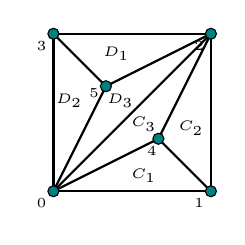
\begin{tikzpicture} 

%\draw[fill=gray!23,gray!23](0,0) rectangle (2.5,2.5);
%\draw[step=0.5cm,gray,very thin] (0,0) grid (2.5,2.5); %background grid

%ielx=1,iely=1,low
\draw[thick] (0,0)--(1.33333,0.66667);
\draw[thick] (2,0)--(1.33333,0.66667);
\draw[thick] (2,2)--(1.33333,0.66667);
%ielx=1,iely=1,high
\draw[thick] (0,0)--(0.666667,1.3333);
\draw[thick] (0,2)--(0.666667,1.3333);
\draw[thick] (2,2)--(0.666667,1.3333);

\draw[thick] (0,0) -- (2,0) -- (2,2) -- (0,2) -- cycle; 
\draw[thick] (0,0) -- (2,2) ; %diag

%\draw[thick] (6,0) -- (4,2) -- (6,4) ; 
\draw[black,fill=teal] ( 0.000000 , 0.000000)     circle (2pt); 
\node[] at ( -0.150000, -0.150000 ) {\tiny 0 }; 
\draw[black,fill=teal] ( 2.000000 , 0.000000)     circle (2pt); 
\node[] at ( 1.850000, -0.150000 ) {\tiny 1 }; 
\draw[black,fill=teal] ( 0.000000 , 2.000000)     circle (2pt); 
\node[] at ( -0.150000, 1.850000 ) {\tiny 3 }; 
\draw[black,fill=teal] ( 2.000000 , 2.000000)     circle (2pt); 
\node[] at ( 1.850000, 1.850000 ) {\tiny 2 }; 
\draw[black,fill=teal] ( 1.333333 , 0.666667)     circle (2pt); 
\node[] at ( 1.25, 0.516667 ) {\tiny 4 }; 
\draw[black,fill=teal] ( 0.666667 , 1.333333)     circle (2pt); 
\node[] at ( 0.516667, 1.25 ) {\tiny 5 }; 

\node[] at ( 1.15,0.2 ) {\tiny $C_1$ }; 
\node[] at ( 1.75,0.8 ) {\tiny $C_2$ }; 
\node[] at ( 1.15,0.85 ) {\tiny $C_3$ }; 

\node[] at ( 0.8,1.75 ) {\tiny $D_1$ }; 
\node[] at ( 0.2,1.15 ) {\tiny $D_2$ }; 
\node[] at ( 0.85,1.15 ) {\tiny $D_3$ }; 

\end{tikzpicture} 
\end{center} 

